\documentclass{article}

% For figures
\usepackage{graphicx} % more modern
\usepackage{subfigure} 
\usepackage{amsfonts}

% For citations
% \usepackage{natbib}

% For algorithms
\usepackage{algorithm}
\usepackage{algorithmic}

\usepackage{hyperref}

% Packages hyperref and algorithmic misbehave sometimes.  We can fix
% this with the following command.
\newcommand{\theHalgorithm}{\arabic{algorithm}}

% \usepackage{sty/icml2013} 
% Employ this version of the ``usepackage'' statement after the paper has
% been accepted, when creating the final version.  This will set the
% note in the first column to ``Proceedings of the...''
\usepackage[accepted]{sty/icml2013}


% The \icmltitle you define below is probably too long as a header.
% Therefore, a short form for the running title is supplied here:
\icmltitlerunning{Clustering and Topic Discovery in Gene Expression Data}

\begin{document} 

\twocolumn[
\icmltitle{Bayesian Clustering and Topic Discovery: \\ 
           Adventures with Gene Expression Data}

% It is OKAY to include author information, even for blind
% submissions: the style file will automatically remove it for you
% unless you've provided the [accepted] option to the icml2013
% package.
\icmlauthor{Karren Dai Yang, Skanda Koppula}{\{karren, skoppula\}@mit.edu}
\icmladdress{Massachusetts Institute of Technology,
            Cambridge, MA 02139 USA}

\icmlkeywords{topic models, bayesian clustering, gene expression, gene modules}

\vskip 0.3in
]

\section{Introduction}
\label{intro}
Tumors cell lines are composed of different sub-populations of cells which often exhibit shared patterns of gene expression. Biologists are interested in two key questions: given gene expressions values, (1) can we identify cell clusterings, and (2) can we identify clusters of biologically-related genes? Our goal with this project was to answer both these two questions using Bayesian methods.

In brief, we explored the use of three Bayesian clustering methods (a vanilla mixture, integrated topic-mixture, and non-parametric models) to address the first question, and two topic models (vanilla and a dynamic-topic LDA) to address the second. 

\subsection{Description of Data}
Using a contemporary gene sequencing machine, we obtained samples of single-cell RNA-sequencing data (scRNA-seq) taken from tumors in mice. Our data consisted of the expression values of 22,712 genes for each of 4645 cells. In total, the dataset amounted to 0.86 GB, presenting significant computational challenges when attempting posterior estimation. Apart from a few computational tricks (online inference, multi-core parallelization), for most methods, we pruned non-informative genes from the dataset, ranking based on the deviation in value across cells \footnote{We recognize that this can bias towards noisy genes. We favor this method because it is simple and easy to implement, and a practice used in literature \cite{pruning}}. The Seurat biological toolkit in R was also used for the purpose of low-variance feature selection \cite{seurat}. We eschewed dimensionality reduction techniques such as PCA because of loss of its direct feature interpretability. Prior researchers have labeled the cells in our dataset; there are a total of 9 cell categories. The complete dataset, as well our preprocessed and pruned versions, are openly available \cite{dataset}.

\subsection{Prior work}
Prior research has explored the use of various computational techniques to analyze gene expression data. Most commonly, Spearman and Pearson correlation metrics are frequently used infer sets of genes that cluster together \cite{profiling, nature}. Other techniques, including PCA followed by linear regression, has been used for expression-based cell clustering \cite{transcriptomics}. Yu et al. propose an unsupervised classifier ensemble as another approach to cell clustering \cite{consensus}. 

More Bayesian approaches have also been tried in prior work from the Pe'er lab. \cite{bayesge2} uses a Heirarchical Dirichlet Mixture Model to learn cell clusterings. \cite{bayesge1} builds on this to jointly learn optimal normalization pre-processing of the data. Bayesian networks have also been used in an attempt to learn gene dependencies from expression data \cite{bayesge3}. Our work uses different models to explore gene expression data, but where appropriate (e.g. in mixture models in Section~\ref{mmsec}), we compare results.

\subsection{Structure of Report}
We first discuss our experiments using Bayesian topic models to discover related sets of genes in a 'topic': LDA in Section~\ref{ldasec} and Dynamic Time Models in Section~\ref{dtmsec}. Then, we discuss our experiments in clustering: Dirichlet Mixtures in Section~\ref{mmsec}, Integrated Topic-Clustering in Section~\ref{intsec}, and non-parametric models in Section~\ref{nonparametricsec}. We conclude our paper with our observations from across all our studies. 

For the purpose of reproducibility, all code can be found at \url{https://github.com/skoppula/882}.

\section{Latent Dirichlet Allocation} 
\label{ldasec}
\subsection{Model Description} 
In the generative process for LDA, the topic assigned to each word is a drawn from the document's topic distribution. The identity of the word is drawn from topic's word distribution. Assuming the reader is familiar with LDA, we relegate further details and formalization of the model to \cite{LDA}.

In the context of analyzing gene expression data, we are interested in discovering 'topics' that comprise of a set of top-$N$ genes within the topic distribution that are biologically related. For example, together the genes may direct a specific chemical function in a cell. Biologists denote such sets of genes as 'gene modules' which can be cross-referenced with existing gene module databases.

\subsection{Implementation} 
A first attempt using the built-in Python \texttt{lda} package resulting in early memory overflows during what we suspect was pre-allocation of per-document variables. The source code was not available, so we had few clues.

We switched to two open-source implementations: an online mean-field variational Bayes for posterior estimation \cite{ovb}, and a broken \texttt{C++} Gibbs sampler for LDA \cite{plda}. 

\nocite{online}

We fixed portions of the sampler to compile properly and extended the sampler to run across four cores. Details of our sampling procedure can be found in Appendix~\ref{ldaappendix}. We compared these two posterior estimation approaches using our entire dataset, using a 10\% held-out testing partition. We experimented using $k=5, 10, 25, 50$ topics. We did not require dataset pruning after these optimizations.

\subsection{Experiments} 
In lieu of intrusion testing, we evaluated the interpretability of our topics (ranked lists of genes) using using hypergeometric tests \cite{hg}. In brief, this determines the probability that our sets of genes would be clustered together in accordance to with existing collections of genes catalogued by biologists in the gene module database \texttt{MSigDB} \cite{msigdb}.

Figure~\ref{fig:pathways} in the Appendix shows gene module matches in \texttt{MSigDB} for which the $p$-value of the match is at least less than 0.3. Notice that models with more topics tended to have more matches with higher significance. The $p$-values in our tests do \textit{not} factor for multiple hypothesis corrections, so at the moment we are only using them as relative measures of model quality.

It is validating to see that many of the similar modules, such as the \texttt{BRCA1} and \texttt{DOXORUBICIN}, are cancer related, given that our expression assay was from tumor cells.

Extracting the parameters of each model, we calculated log-likelihood on our held-out test set. This is shown in Figure \ref{fig:ll}. We found that for this dataset increasing the topic count increases log-likelihood, roughly linear from 5 to 50. Further experiments will need to test at what point log-likelihood drops off; this is one way to optimize the number of topics.

\begin{figure}
    \centering
    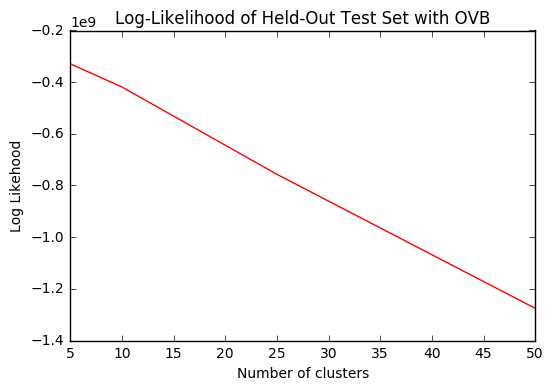
\includegraphics[width=0.4\textwidth]{figs/ll}
    \caption{Log-likelihood of the held-out testing set across numbers of topics. Higher topic sizes are explored in later models.}
    \label{fig:ll}
\vskip -0.2in
\end{figure}


As an interesting aside, Figure \ref{fig:time} shows the time until inference completion (collected during our experiments). Gibbs appears to scale poorly with the parameter dimensionality, in contrast to online variational Bayes \footnote{It is important to note that comparing the magnitude of the time to complete inference in Figure~\ref{fig:time} is not particularly meaningful; as described in Appendix~\ref{ldaappendix}, we chose a reasonable guess for the number of iterations
and optimization threshold after which to stop estimation}. 

\begin{figure}
    \centering
    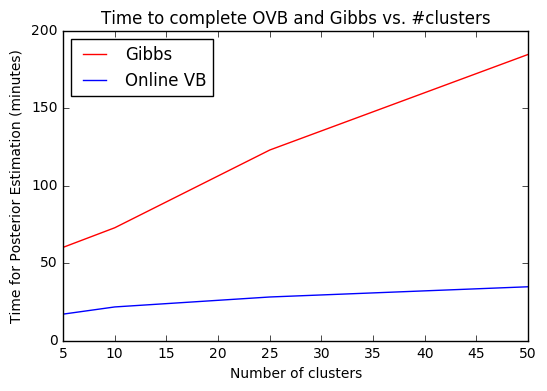
\includegraphics[width=0.4\textwidth]{figs/time}
    \caption{Comparison of the running times of each of the posterior estimation methods across various numbers of topics. Termination conditions across all runs were constant, and described in Appendix~\ref{ldaappendix}}
    \label{fig:time}
\end{figure}

Posterior predictive checks to test the mutual information between the each cell and its words' topics is something that we did not have time, but would be interesting to examine. It's not clear that this independence assumption is true in the context of gene expression data, because of cross-talk and regulatory mechanisms between gene modules.

\section{Dynamic Topic Model} 
\label{dtmsec}
\subsection{Model Description} 
As tumor cells proliferate, they undergo a process called \textit{differentiation}. The set of cells types during tumor emergence may differ from the set of types expressed days later. Correspondingly, patterns of gene expression may also change over time. The set of gene modules expressed in the cells, or the composition of each gene module (topic), may also change.

To capture these evolving topics, we look to dynamic topic models \cite{dtm}. In brief, dynamic topic models establish a conditional distribution over the hyperparameters $\alpha$ and $\beta$, that govern the document's topic distribution and topic's word distribution, respectively. The distribution over each hyperparameter is conditioned on the prior in the previous time step, allowing changes to topic composition and assignment. This can be seen graphically in the plate
model in Figure~\ref{fig:dtmplate}. For convenience, we provide a concise description of the generative process for the implemented heirarchical model for a time slice $t$ in Appendix~\ref{dtmappendix}.

\begin{figure}[h]
    \vspace{-0.1in}
    \centering
    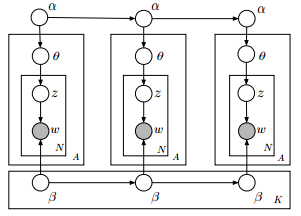
\includegraphics[width=0.4\textwidth]{figs/dtmplate}
    \caption{Plate diagram for the Dynamic Topic Model. Reproduced from \cite{dtm}.}
    \label{fig:dtmplate}
    \vspace{-0.1in}
\end{figure}

Note that in contrast to LDA, dynamic topic models use a logistic-normal to express proportion uncertainty. This is stated more explicitly in Appendix~\ref{dtmappendix}.

\subsection{Implementation} 

Unfortunately, due to the non-conjugacy of the Gaussian/Multinomial in our logistic-normal setup, integrating out parameters for any sort of Gibbs sampling becomes hard. Instead, the original DTM paper uses a variational approximation based on a Kalman filter, that preserves time dependencies, unlike a mean-field approximation.

Re-implementing the variational approximation, while educational and interesting, would be a project of itself, so our first attempt in employing dynamic time models to our gene expression data re-used the Kalman Filter-based variational inference used by the original authors, published recently by the Blei Lab \cite{dtmbleigit}. The results we show in the subsequent section are using a wrapper we've implemented around the group's inference code.

The authors stumbled upon a recent arXiv pre-print that proposed a set of sampler update rules to create a correct DTM Gibbs sampler \cite{sdtm}. Using the probabalistic programming framework \texttt{Edward}, and modifying the in-built sampler to follow these updates, we were able to obtain a working Gibbs-sampler for sample time-sliced data for a dynamic topic model defined in Edward \cite{edward}. While we don't have time to conduct benchmarks or re-run our results right now, after verifying that results are consistent, the authors hope to submit a merge for this Edward sketch into the mainstream Edward examples library this coming summer.

\subsection{Experiments} 
We subdivided our data into three seperate time slices, and pruned each slice, retaining the top 20\% of high-variance genes. We experimented using $k=15$, $30$, and $50$ topics.

Similar to our analysis in Section~\ref{ldasec}, we used the hypergeometric test to evaluate interpretability. 

Figure~\ref{fig:pathwaysdtm} in the Appendix shows gene module matches for which the $p$-value is less than 0.3, across the three time slices and the three topic count sizes. Interestingly, we notice a very different set of matched gene modules, with exception of the \texttt{KLF1} module\footnote{This could very well be a result of our dataset pruning, which we did to keep inference runtimes manageable}. Like before, we notice that some of the identified topics are relevant to tumor cells:
\texttt{ST\_TUMOR\_NECROSIS\_FACTOR\_PATHWAY} and \texttt{WEST\_ADRENOCORTICAL\_TUMOR\_MARKERS\_UP} to name the two most prominent topics.

We do not see that much variation across time-slices, demonstrating that our time-slice partitions are largely uniform. For example, for model $k=50$, we see that topic 20 consistently matches with MSigDB module \texttt{PILON\_KLF1\_TARGETS\_UP}, suggesting that its gene composition is not varying.

Models with more topics tended to have more matches with higher significance. But again, the $p$-values in our tests do \textit{not} factor for multiple hypothesis corrections, so at the moment we are only using them as relative measures of model quality.

After extracting the mode of learned parameters, we evaluated the log-likelihood of our held-out test set, also partitioned by time. This is shown in Figure \ref{fig:lldtm}. We find a leveling of log-likelihood after $k=30$.

\begin{figure}
    \centering
    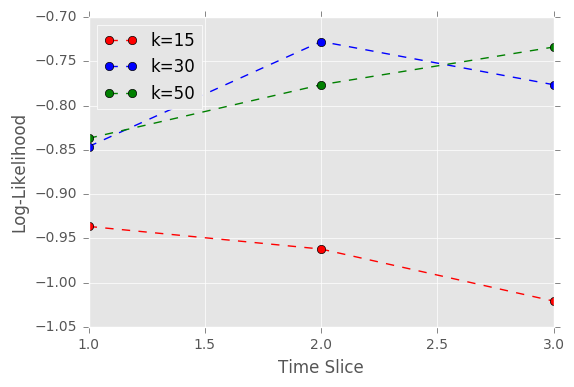
\includegraphics[width=0.4\textwidth]{figs/lldtm}
    \caption{Log-likelihood of the held-out testing set across our time slices for varying numbers of topics.}
    \label{fig:lldtm}
\vskip -0.2in
\end{figure}

With more time, we would ideally repeat the experiments to obtain confidence intervals on these experiments, and examine the gene-module/cell/time-slice mutual information.

\section{Dirichlet Mixture Model} 
\label{mmsec}
\subsection{Model Description} 
\subsection{Implementation} 
\subsection{Experiments}  
- comparison with pe'er paper



\section{Integrated Topic-Clustering Model} 
\label{intsec}
\subsection{Model Description} 
\subsection{Implementation} 
\subsection{Experiments} 



\section{Non-parametric Models: IBP and HDP} 
\label{nonparametricsec}
\subsection{Model Description} 
\subsection{Implementation} 
\subsection{Experiments} 

\section{Conclusions} 
\label{nonparametricsec}

% In the unusual situation where you want a paper to appear in the
% references without citing it in the main text, use \nocite
% \nocite{langley00}

\bibliography{citations}
\bibliographystyle{sty/icml2013}


\section{Appendix} 

\subsection{Breakdown of Work}
The implementation(s) and experiments involving LDA, Dirichlet Mixtures, and Dynamic Time Model was completed by SK (Section~\ref{ldasec}, Section~\ref{mmsec}, and Section~\ref{dtmsec}). KY completed the implementations and experiments involved Integrated Topic-Clustering, Non-Parametric models, and the shared gene enrichment test implementation (Section~\ref{intsec} and Section~\ref{nonparametricsec}). The authors contributed equally in this work.

\subsection{Latent Dirichlet Allocation}
\label{ldaappendix}
For our Gibb's sampler, we had a fixed burn-in of number of samples (200), a fixed number of sampling iterations after that (500). We didn't extensively explore varying these values, but trying out significantly more iterations (700) didn't seem to change the topic's word distributions significantly. There was one sampling chain on each of four cores.

\begin{figure*}
    \centering
    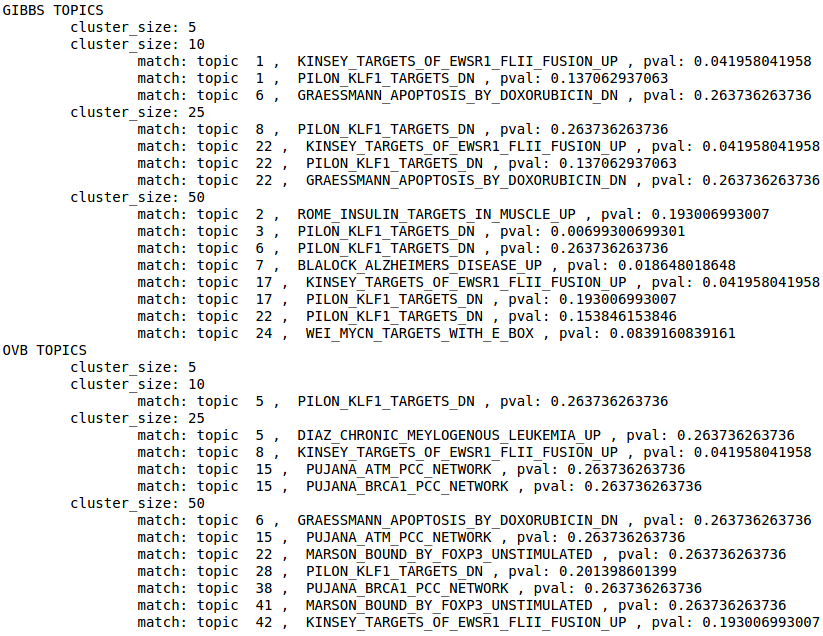
\includegraphics[width=1\textwidth]{figs/pathways}
    \caption{Matches between the gene collections found in LDA topics and published gene sets in \texttt{MSigDB}. `Cluster size' refers to the number of topics in the model}
    \label{fig:pathways}
\end{figure*}

\subsection{Dynamic Topic Model}
\label{dtmappendix}
Here is a description of the generative process for our dynamic topic model:
\begin{enumerate}
    \item Draw a new topic composition hyperparameter \\ $\beta \leftarrow \mathbb{N}(\beta_{t-1}, \sigma I^2)$
    \item Draw a new document composition hyperparameter \\ $\alpha \leftarrow \mathbb{N}(\alpha_{t-1}, \delta I^2)$
    \item For each document: 
    \begin{enumerate}
        \item Draw a new document topic distribution \\ $\theta \leftarrow \pi(\mathbb{N}(\alpha_t))$
        \item For every word in the document:
        \begin{enumerate}
            \item Draw the word topic assignment \\ $Z \leftarrow$ Mult$(\theta)$
            \item Draw the word identity \\ $Z \leftarrow$ Mult$(\pi(\beta_{t,z}))$
        \end{enumerate}
    \end{enumerate}
\end{enumerate}
Here, $\pi(x_i)$ is the softmax function $\frac{exp(x_i)}{\sum_k exp(x_k)}$ \cite{dtm}.

\begin{figure*}
    \centering
    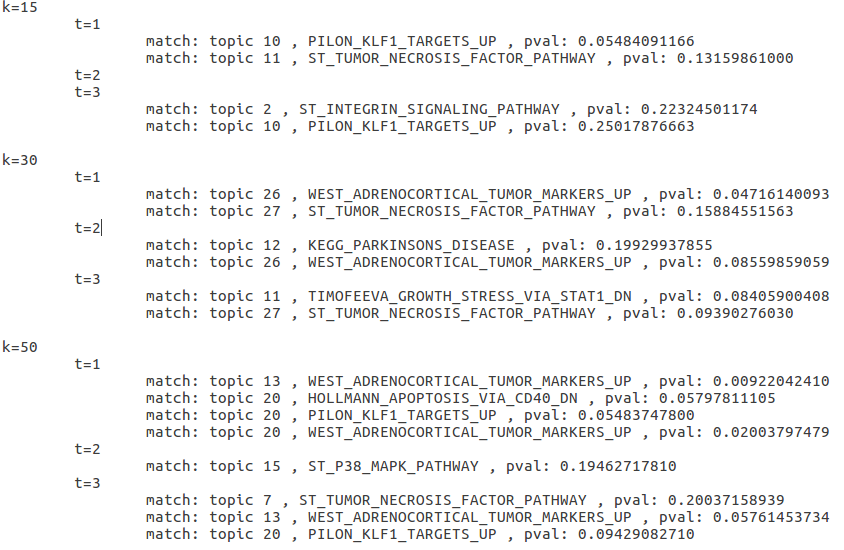
\includegraphics[width=1\textwidth]{figs/pathwaysdtm}
    \caption{Matches between the gene collections found using a dynamic topic model and published gene sets in \texttt{MSigDB}. $k$ refers to the number of topics in the model. $t$ refers to the time slice in the model.}
    \label{fig:pathwaysdtm}
\end{figure*}

\end{document} 
